\chapter{Introduction}

\section{Calorimetry in high-energy physics} % SAGAR
Calorimetry is a technique used in nuclear and particle physics to describe the detection and measurement of particles by complete absorption in a block of matter. The measurement process associated with calorimetry is destructive in nature, that is, once the particle of interest has been absorbed and its properties have been characterized by the calorimeter, it is no longer available to be detected by other devices. \\

A calorimeter used in a high energy physics experiment is way more sophisticated and sensitive than a calorimeter typically used in standard thermodynamics experiments like measuring the heat of a reaction. The order of magnitude of the unit of energy measured in a calorimeter in the standard thermodynamic context varies around 1-1000 Joules. However, the calorimeters used in high energy physics are more sensitive. In modern particle accelerator experiments, the most energetic particles are measured in terms of TeV, where 1 TeV = 10\textsuperscript{7} eV, and around 6.24 × 10\textsuperscript{6 } TeV = 1 J. \\ 

Calorimeters are broadly categorized as either electromagnetic or hadronic calorimeters. As the names suggest, the former are used for the detection of photons and electrons through interactions mediated by the electromagnetic force, whereas, the latter are used for the detection of hadrons through interactions mediated by the strong and electromagnetic forces. \\

In essence, a primary particle passing through a calorimeter interacts with the calorimeter matter producing a 'particle shower', which can be described as the production of many secondary particles that are generated from the interaction process of the primary particle and the consecutive particles with the calorimeter, till the energy of the shower particles goes below a certain threshold, and they start getting completely absorbed instead of producing further particles. Thus, it can also be stated that in the direction of the particle, the energy of the shower particles shows a continuous degradation. In general, a hadronic shower is wider in shape (encompasses a larger calorimeter area) than an electromagnetic shower. \\

Based on the construction of calorimeters, they can be further characterized into homogenous and sampling calorimeters. The latter refer to a class of calorimeters that have their entire volume of matter dedicated to degrading the particle energy as well as producing signals. Sampling calorimeters, on the other hand, have alternate volumes of active and passive media that are used for producing signals and degrading particle energy, respectively. In general, the passive medium is a high-density medium such as copper, lead, uranium, iron, etc. There are different ways in which the active and passive media can be arranged with respect to one another. For example, the active medium layers can be in the same direction as the incoming particles or perpendicular to them. Some of the different geometries that can be made can resemble an accordion or a tile. \\

In most modern particle physics experiments, the mechanisms through which calorimeter signals are produced include scintillation, Cherenkov radiation, and ionization. When an incident particle passes through the calorimeter medium, it can lose energy by exciting the constituent atoms and molecules of the medium. When these atoms and molecules go back to their de-excited states, they release that energy in the form of photons. These photons can then be directed toward a photon counter via an optical fiber to get electric signals. On the other hand, if the incident particle is traveling at a speed faster than the speed of light in the calorimeter medium, it will emit Cherenkov photons, which can be collected. Calorimeters based on this principle have a very fast response as there is no delay in Cherenkov photon detection such as that associated with the de-excitation of excited states of atoms and molecules. Lastly, there is also a possibility of the incident particle knocking off electrons from the atoms and molecules of the calorimeter medium. In this case, an electron-ion pair is formed. The signal, in this case, is observed when the charged particles are collected by electrodes with an applied potential difference between them, creating an electric field to drift them apart. In the case of semiconductor detectors, the signals are observed by the creation of electron-hole pairs. They have better energy resolution since an energy of around 3.6 eV is required to create an electron-hole pair in silicon, which is one order of magnitude less than the energy required to ionize gases, and two orders of magnitude less than the energy required to produce a single photoelectron in the photon counters used to detect the scintillation photons. \\

Keeping the physics goals of the experiment in mind, the design of a calorimeter includes the following aspects:
\begin{itemize}
    \item Whether the calorimeter would be a sampling or a homogenous calorimeter.
    \item What should be the material used for its different segments.
    \item How would the different segments be geometrically aligned with respect to one another.
    \item Whether the calorimeter is designed to primarily detect electrons, hadrons or other particles.
    \item What mechanism would be used for particle detection.
\end{itemize}

If properly designed, a calorimeter would account for all the requirements of the experiment to achieve its goals. \\

R. Wigman's book on Calorimetry \cite{principles} has been used to obtain most of the information in this section. It can be referred to for exhaustive information about calorimetry in contemporary particle physics.

\section{Electron-Ion Collider Experiment } % SIMRAN
The Electron-Ion Collider (EIC) is a new and innovative nuclear physics experiment planned for construction at Brookhaven National Laboratory on Long Island, New York which will be ready to operate by 2030. 

\begin{figure}[H]
        \centering
		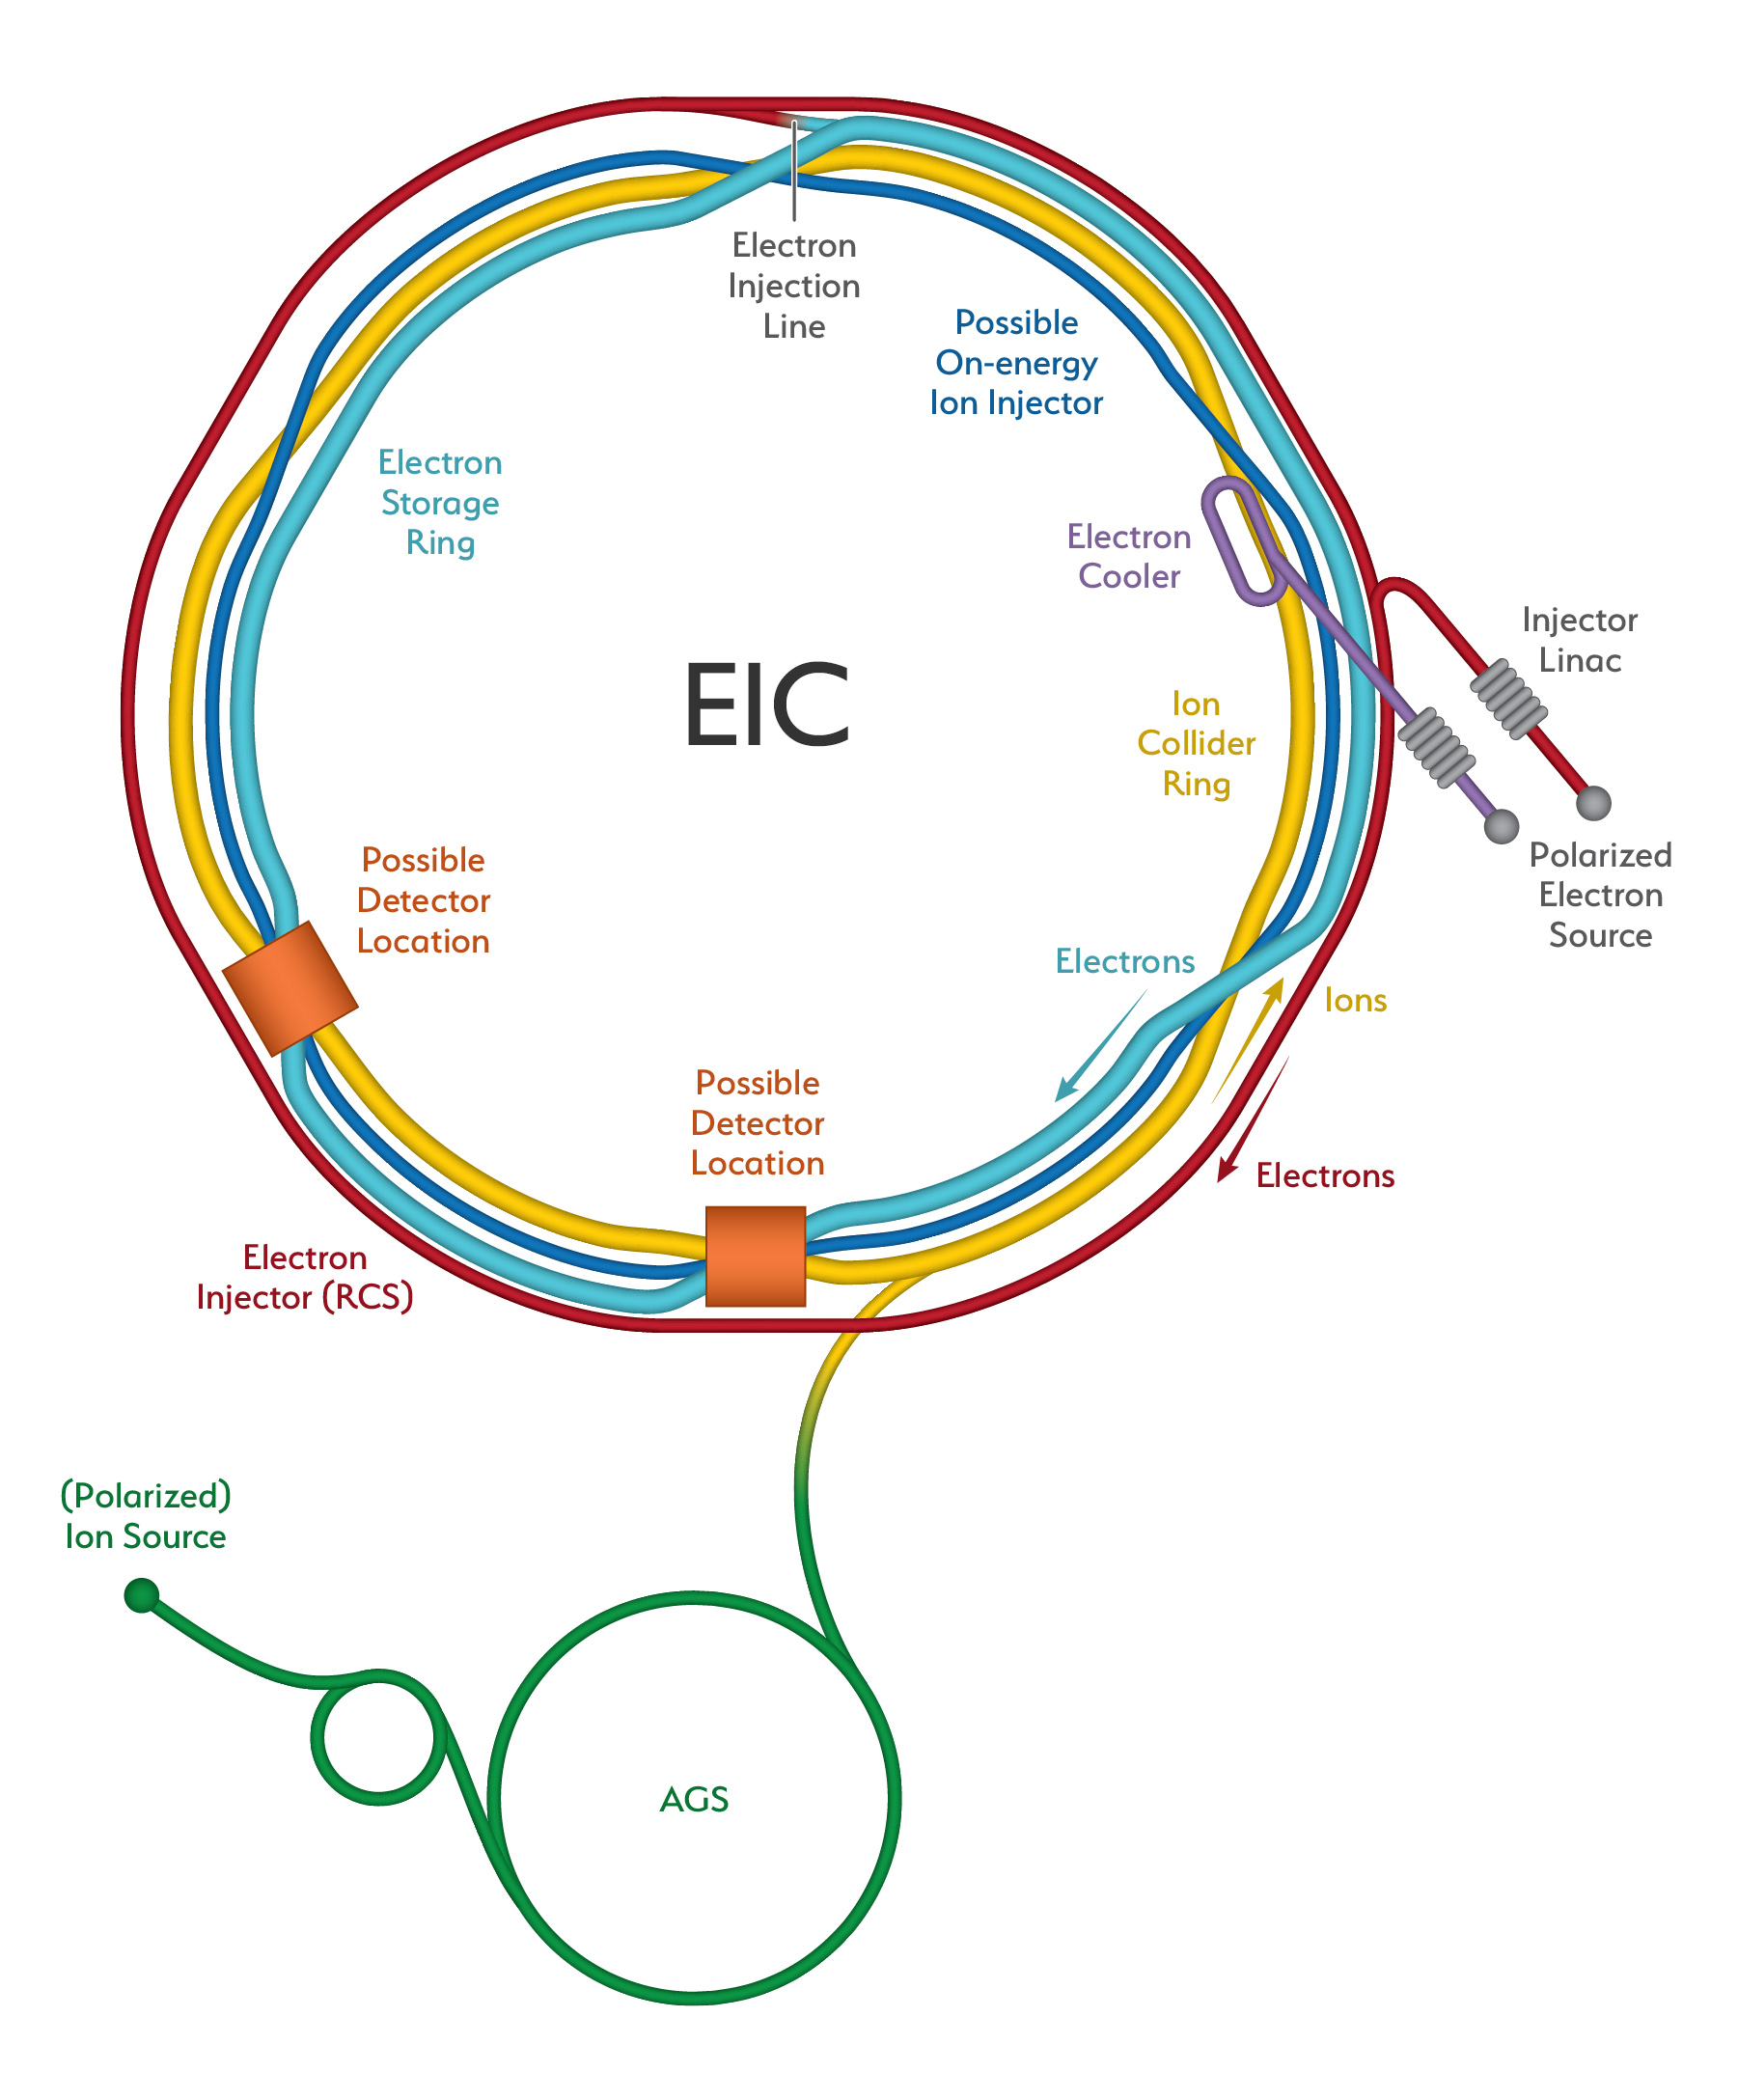
\includegraphics[width=0.5\linewidth]{group1/eic-hr.jpg}
		\caption{Schematic design for EIC accelerator}
		\label{fig:g1_ch1_img1}
\end{figure} 

Figure \ref{fig:g1_ch1_img1}, as obtained from \cite{yellowreport2021}, shows the schematic design for the EIC accelerator. This experiment aims to probe the internal structure of protons, neutrons, and atomic nuclei by colliding polarized beams of highly-energetic electrons with highly-energetic protons or ion beams. EIC aims for center of mass energies in the range of $20-100$ GeV and will operate at high collision luminosity for electrons and nucleons \cite{yellowreport2021}. This would help in studying the new realms within nuclear physics by shedding light on the properties of nuclear forces and how nucleons are bound inside the nucleus.

\subsection{Long-term Goals}

The main physics issues that will be addressed by EIC are as follows:
\begin{enumerate}
    \item The mechanism of origin of mass and spin of the nucleus from quarks and gluons and their corresponding interactions.
    \item The distribution of partons within the nucleus in momentum and position space.
    \item The mechanism of nuclear binding and origin of confined hadronic states from interactions of color-charged partons and jets, with a nuclear medium.
\end{enumerate}

Figure \ref{fig:g1_ch1_img1} visualizes the planned accelerator for EIC. This scheme is based on the existing accelerator system at RHIC.

\subsection{EIC Calorimetry Requirements}
\begin{figure}[H]
        \centering
		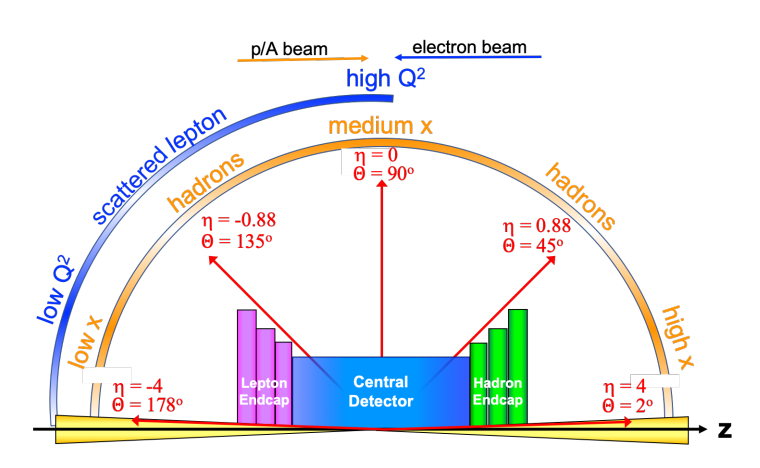
\includegraphics[width=0.5\linewidth]{group1/EIC_1.png}
		\caption{Schematic design for EIC accelerator}
		\label{fig:g1_ch1_img2}
\end{figure}
Figure \ref{fig:g1_ch1_img2}, as obtained from \cite{yellowreport2021}, shows the pseudorapidity and polar angle coverage of the EIC physics program in $x - Q^2$ space. The detector needs to encompass the pseudorapidity region from -4 to 4. In this region, the calorimeter configuration needs to cover the electron end-cap, barrel, and hadron end-cap in order to measure the energies of the incident hadrons and leptons.

There is a need for electromagnetic and hadronic calorimetry for the above regions according to the following energy resolution specifications:
\begin{enumerate}
    \item For the electron-going or backward region, an excellent electromagnetic energy resolution is required. The minimum requirement is $$\sigma _E/E \approx (1-3)\% \oplus 2\%/\sqrt{E} $$
    \item For the barrel region, a good electromagnetic energy resolution is required. The minimum requirement is $$\sigma _E/E \approx (1-3)\% \oplus 10\%/\sqrt{E} $$
    \item For the hadron-going or forward region, good hadronic calorimeter resolution is required. The minimum requirement is $$\sigma _E/E \approx 10\% \oplus 50\%/\sqrt{E} $$
\end{enumerate}

The detailed energy resolution requirements for EIC calorimeters are as follows:
\begin{enumerate}
    \item Electromagnetic Calorimetry: For the study of physics processes, there is a need for excellent energy resolution for incident electrons, especially in the backward region with $\eta < -2$. Table \ref{table:g1_ch1_t1} shows the required energy resolution parameters spanning the rapidity region of $-4 < \eta < 4$.
        \begin{table}[H]
        \centering
        \begin{tabular}{ | m{8em} | m{1.5cm}| m{1.5cm} | m{1.5cm} | m{1.5cm} |} 
        \hline
        $\eta $ & -4 to -2 & -2 to -1 & -1 to 1 & 1 to 4 \\ 
        \hline
        $\sigma _E/E . \sqrt{E/1 GeV}$ & 2\% & 7\% & 10-12\% & 10-12\%\\ 
        \hline
        \end{tabular}
        \caption{The electromagnetic calorimeter (ECAL) energy resolution requirements}
        \label{table:g1_ch1_t1}
        \end{table}
        
    \item Hadronic Calorimetry: The main consideration for the EIC hadronic calorimetry is its ability to reconstruct energy of jets precisely along with the detection of hardons which mainly go towards the forward region. The jet fragments cover the range of $-3.5 < \eta < 3.5$ and the required energy resolution of hadronic calorimetry for their detection is summarized in table \ref{table:g1_ch1_t2}.
      
        \begin{table}[H]
        \centering
        \begin{tabular}{|c|c|c|c|c|}
        \hline
        \multirow{2}{*}{$\eta$} & \multicolumn{2}{|c|}{EIC Specifications} & \multicolumn{2}{|c|}{Conservative option} \\ 
        \hhline{~----}
        & $\sigma_E/E (\%)$ & $E_{min} (MeV)$ & $\sigma_E/E (\%)$ & $E_{min} (MeV)$ \\
        \hline
        $-3.5$ to $-1.0$ & $45/\sqrt{E}+7$ & $500$ & $50/\sqrt{E}+10$ & $500$\\
        \hline
        $-1.0$ to $+1.0$ & $85/\sqrt{E}+7$ & $500$ & $100/\sqrt{E}+10$ & $500$\\
        \hline
        $+1.0$ to $+3.5$ & $35/\sqrt{E}$ & $500$ & $50/\sqrt{E}+10$ & $500$\\
        \hline
        \end{tabular}
        \caption{The hadronic calorimeter (HCAL) energy resolution requirements}
        \label{table:g1_ch1_t2}
        \end{table}
\end{enumerate}

\section{Fun4All: EIC simulation framework} % SIDDHANT

Fun4All is a C++ based framework which specializes in running raw data reconstruction, analysis, simulations and embedding. The simulations are GEANT4 based and are fully integrated into the analysis chain in the form of a Reconstruction Module. An important aspect of fun4All is its modularity, that is, the code relevant to a particular detector is self contained and not reliant on any other detectors. 

Fun4All is entirely configured with Root macros. Figure \ref{fig:fun4all} shows the overall blockdiagram of the structure of the fun4All framework as obtained from \cite{fun4all}.

\begin{figure}[H]
        \centering
		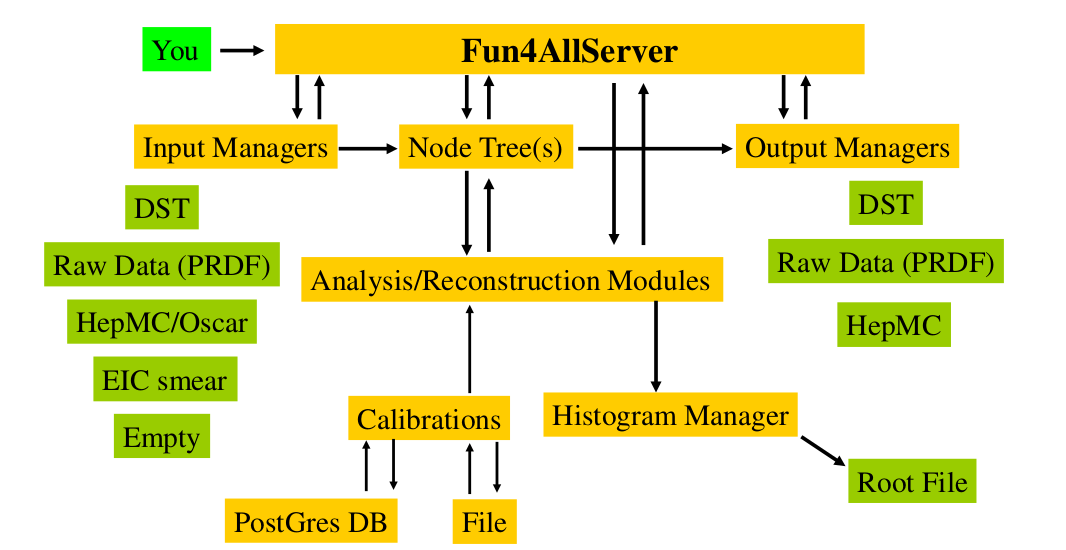
\includegraphics[width=1\linewidth]{Chapters/fun4All.png}
		\caption{Structure of fun4All framework}
		\label{fig:fun4all}
\end{figure}

Some of the main features of Fun4All include:
\begin{itemize}
    \item It can read input files of different types.
    \item It can write output files of different types, automatically saving selected data objects.
    \item It can manage many independent Node Trees, which are structures through which the data is organized and made accessible to modules.
    \item It calls analysis and reconstruction modules in the order in which they are registered.
    \item It can make snapshots at any state of the reconstruction or the analysis.
    \item It has access to all the necessary calibrations.
\end{itemize}

There are a couple of event generators that can be used via Fun4All. A few of them are:
\begin{itemize}
    \item Hijing
    \item Pythia6
    \item Pythia8
    \item Sartre
    \item Single Particle Generators
\end{itemize}


